\subsection{Frozen generator diagnostics}
Across ten paired factorial seeds, the optical main effect on validation reconstruction MSE was +0.000002 (95\% CI -0.000027 to +0.000032; Holm-adjusted $p=0.977$). The boundary-and-moment main effect was -0.000071 (95\% CI -0.000124 to -0.000018; adjusted $p=0.064$). The validation-only path reached its lowest mean reconstruction MSE (0.000526) at optical weight 0.0035. The closest Gaussian/heat smoothing control remained 14.1\% from that target and therefore failed the frozen 5\% matching tolerance (Fig.~1). These are development diagnostics, not held-out detector outcomes.

The common-roster quality analysis compared domain morphology, ImageNet-feature distribution, texture, diversity, and automated similarity screens (Fig.~2). Among the five synthetic arms, ND had the largest aggregate distances (PFFD10 6352.973; FID 5.514); the corresponding ranges across NB, NF, NP, and NS were 0.368--6.112 and 0.031--0.633, respectively. These measures were interpreted descriptively: ImageNet features are not domain-calibrated, and the automated screen can neither prove nor exclude memorization. Generated arrays and inherited boxes passed roster alignment, but independent physical label validation was outside scope.

\subsection{Held-out detector utility}
The highest unadjusted mean held-out AP among the eight primary arms was observed for NR (0.652); this ranking was not itself a confirmatory comparison. NP-NB was +0.006 (CI +0.001 to +0.012) and favoured NP over the comparator; NP-NF was -0.001 (CI -0.007 to +0.004) and was compatible with effects in both directions; NP-N1 was -0.008 (CI -0.017 to +0.001) and was compatible with effects in both directions; NP-NR was -0.010 (CI -0.019 to -0.001) and favoured the comparator over NP. Intervals used the same resampled specimens and pipeline indices for every arm and a 98.75\% individual confidence level for the four-comparison family (Fig.~3). The fast pooled-AP implementation agreed with pycocotools in all 50 primary cells before resampling.

\subsection{Sensitivity and internal robustness}
Across the predeclared low-data contrasts, mean NP effects ranged as follows ($n=14$: -0.006 to +0.002; $n=28$: +0.002 to +0.008; $n=56$: -0.007 to +0.010); these 95\% intervals were secondary and descriptive. The three-partition development-cohort grouped out-of-fold effects were NP-NB +0.002 (partition range -0.002 to +0.006); NP-N1 -0.006 (partition range -0.008 to -0.005); NP-NR -0.009 (partition range -0.014 to -0.006). Because those predictions reused the development cohort through grouped out-of-fold construction, they provide an internal robustness check rather than external validation. The validation-only common-64 resolution pathway changed mean AP relative to native-300 evaluation by N1 -0.235, NB -0.209, NP -0.208, NR -0.243; the unavailable 1024-pixel branch was not inferred (Fig.~4).

\begin{figure}[p]
\centering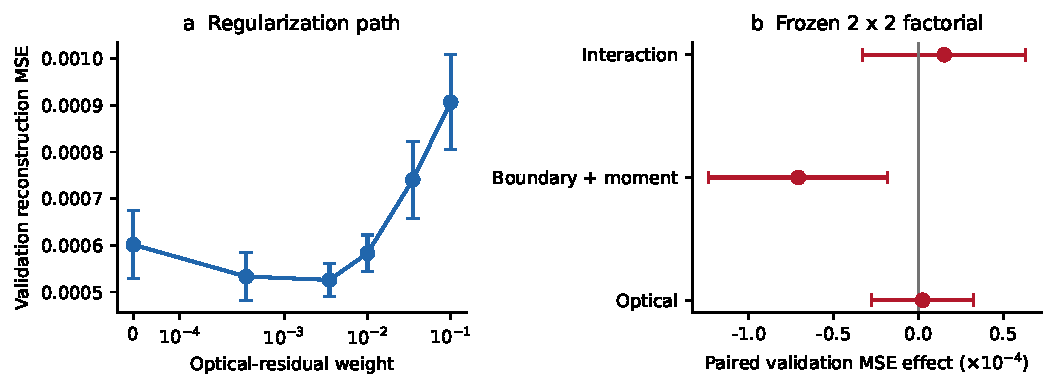
\includegraphics[width=\linewidth]{figures/figure_1_generator_mechanism.pdf}\caption{Generator mechanism diagnostics.}\end{figure}
\begin{figure}[p]
\centering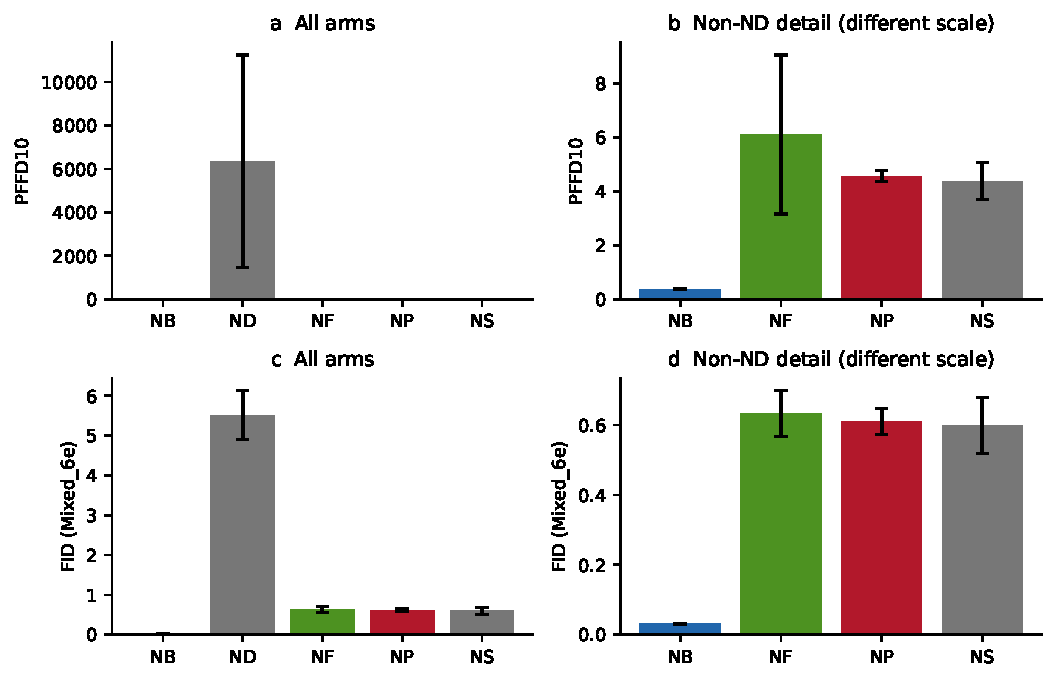
\includegraphics[width=\linewidth]{figures/figure_2_synthetic_quality.pdf}\caption{Synthetic-image quality diagnostics.}\end{figure}
\begin{figure}[p]
\centering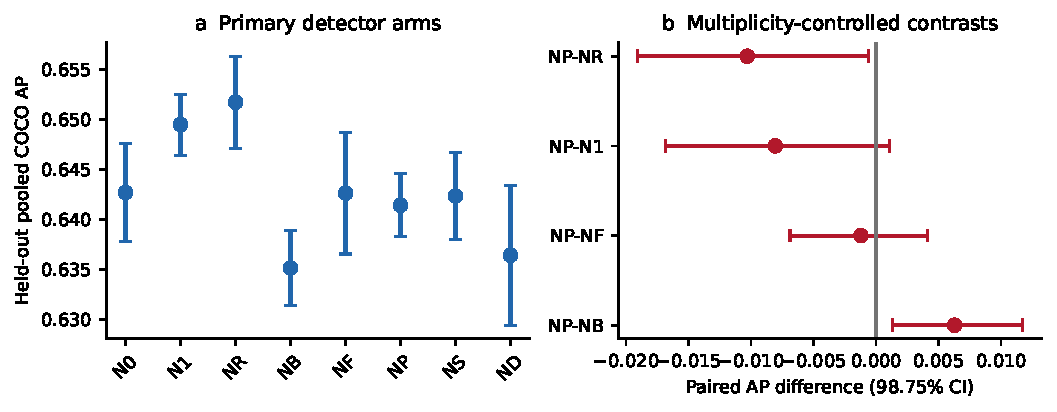
\includegraphics[width=\linewidth]{figures/figure_3_primary_detection.pdf}\caption{Frozen primary detector results.}\end{figure}
\begin{figure}[p]
\centering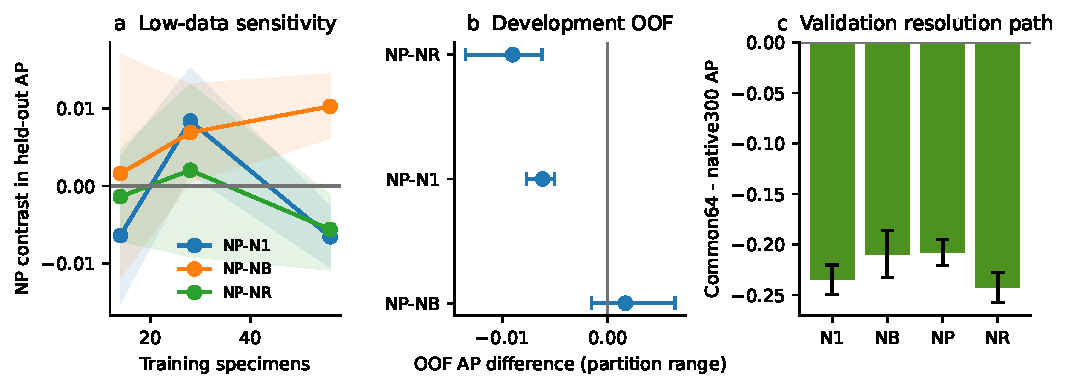
\includegraphics[width=\linewidth]{figures/figure_4_sensitivity.pdf}\caption{Secondary sensitivity analyses.}\end{figure}
